\subsubsection{DTO (Data Transfer Objects)}

\paragraph{Introduzione}
\par Questa sezione descrive le classi che si occupano dei DTO (Data Transfer Objects), ossia design pattern utilizzati per il tasferimento dei dati nell'applicazione.

\paragraph{ResponseStatusEnum} \label{ResponseStatusEnum} 
\begin{figure}[h!]
    \centering
    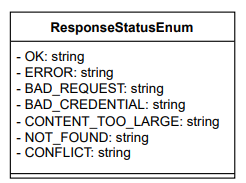
\includegraphics[width=0.30\textwidth]{assets/Backend/response_status_enum.png}
    \caption{Rappresentazione della classe ResponseStatusEnum}
\end{figure}
\par Enumerazione contenente i possibili stati di risposta del sistema.

\paragraph{DictionaryDto} \label{DictionaryDto}
\begin{figure}[h!]
    \centering
    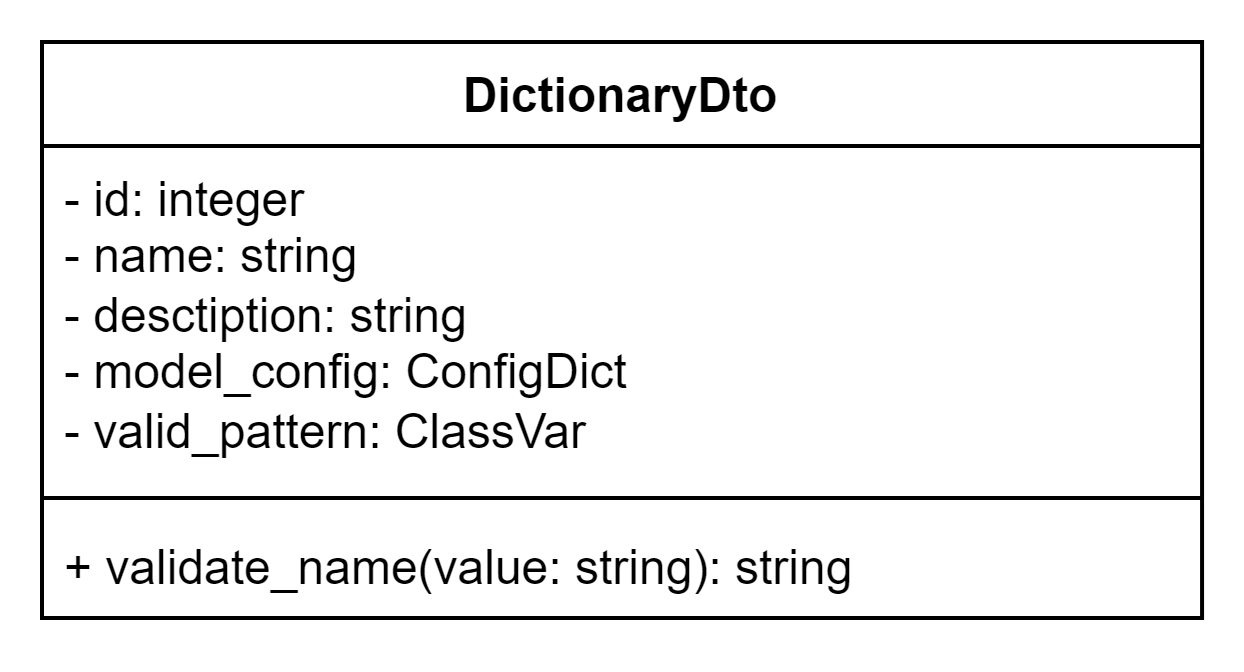
\includegraphics[width=0.40\textwidth]{assets/Backend/dictionary_dto.png}
    \caption{Rappresentazione della classe DictionaryDto}
\end{figure}
\par DTO relativo ai \glossario{dizionari dati}, contenente le informazioni relative a: id, nome, descrizione, configurazione e validazione del pattern

\paragraph{PromptDto} \label{PromptDto}
\begin{figure}[h!]
    \centering
    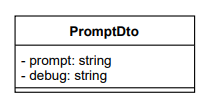
\includegraphics[width=0.30\textwidth]{assets/Backend/prompt_dto.png}
    \caption{Rappresentazione della classe PromptDto}
\end{figure}
\par DTO relativo ai \glossario{prompt} generati. Contiene le informazioni relative al prompt generato e al rispettivo log di debug.

\paragraph{DictionaryPreviewDto} \label{DictionaryPreviewDto}
\begin{figure}[h!]
    \centering
    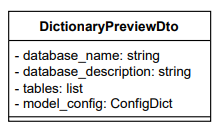
\includegraphics[width=0.30\textwidth]{assets/Backend/dictionary_preview_dto.png}
    \caption{Rappresentazione della classe DictionaryPreviewDto}
  \end{figure}
\par DTO relativo alle anteprime dei dizionari dati, le quali ne mostrano il nome, la descrizione e la lista delle tabelle

\paragraph{LoginDto} \label{LoginDto}
\begin{figure}[h!]
    \centering
    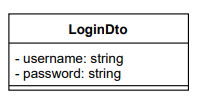
\includegraphics[width=0.30\textwidth]{assets/Backend/login_dto.png}
    \caption{Rappresentazione della classe LoginDto}
  \end{figure}
\par DTO relativo ai login dei tecnici. Includono le informazioni riguardanti lo username e la password per l'accesso.

\paragraph{AdminDto} \label{AdminDto}
\begin{figure}[h!]
    \centering
    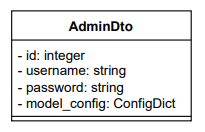
\includegraphics[width=0.30\textwidth]{assets/Backend/admin_dto.png}
    \caption{Rappresentazione della classe AdminDto}
  \end{figure}
\par DTO relativo alle informazioni riguardanti gli amministratori dell'applicativo. Contiene le informazioni relative all'id dell'admin, il suo username e la sua password.

\paragraph{ResponseDto} \label{ResponseDto}
\begin{figure}[h!]
    \centering
    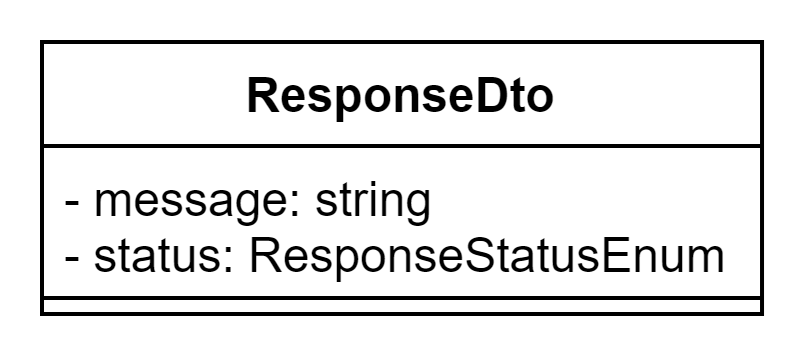
\includegraphics[width=0.30\textwidth]{assets/Backend/response_dto.png}
    \caption{Rappresentazione della classe ResponseDto}
  \end{figure}
\par DTO relativo ai tipi di risposta del sistema, i quali permettono la visualizzazione del problema con un avviso a schermo.

\paragraph{StringDataResponseDto} \label{StringDataResponseDto}
\begin{figure}[h!]
    \centering
    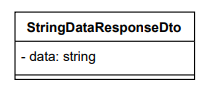
\includegraphics[width=0.30\textwidth]{assets/Backend/string_data_response_dto.png}
    \caption{Rappresentazione della classe StringDataResponseDto}
  \end{figure}
\par FIXME

\paragraph{PromptResponseDto} \label{PromptResponseDto}
\begin{figure}[h!]
    \centering
    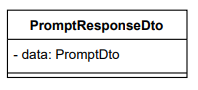
\includegraphics[width=0.30\textwidth]{assets/Backend/prompt_response_dto.png}
    \caption{Rappresentazione della classe PromptResponseDto}
  \end{figure}
\par FIXME

\paragraph{AuthResponseDto} \label{AuthResponseDto}
\begin{figure}[h!]
    \centering
    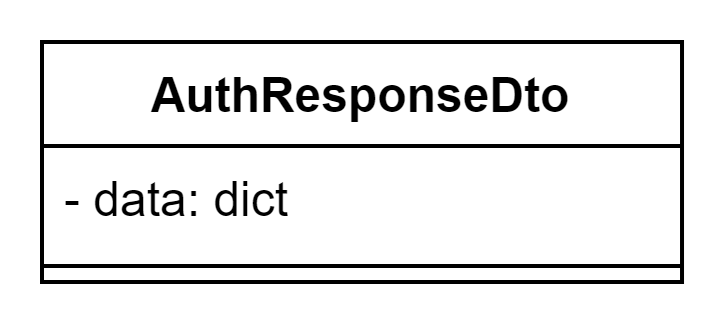
\includegraphics[width=0.30\textwidth]{assets/Backend/auth_response_dto.png}
    \caption{Rappresentazione della classe AuthResponseDto}
  \end{figure}
\par FIXME

\paragraph{DictionaryResponseDto} \label{DictionaryResponseDto}
\begin{figure}[h!]
    \centering
    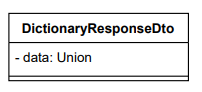
\includegraphics[width=0.30\textwidth]{assets/Backend/dictionary_response_dto.png}
    \caption{Rappresentazione della classe DictionaryResponseDto}
  \end{figure}
\par FIXME